\section{Spécifications}

\subsection{Caractérisation de l'environnement}

Il s'agit dans cette partie de caractériser l'environnement c'est-à-dire de d'identifier les entités interagissant avec le circuit à concevoir et décrire leur évolution à l'aide d'automates.
L'environnement du circuit à concevoir est constitué de N entités :

\begin{itemize}
	\item a
	
\end{itemize}

\subsection{Entrées et sorties du composant}

La caractérisation de l'environnement sous forme d'automates donne les relations d'entrées et sorties du circuit à concevoir avec les diverses entités.
Il est alors possible de présenter de manière structurelle le circuit à concevoir et les entités de l'environnement.

\begin{figure}[H]
	\centering
	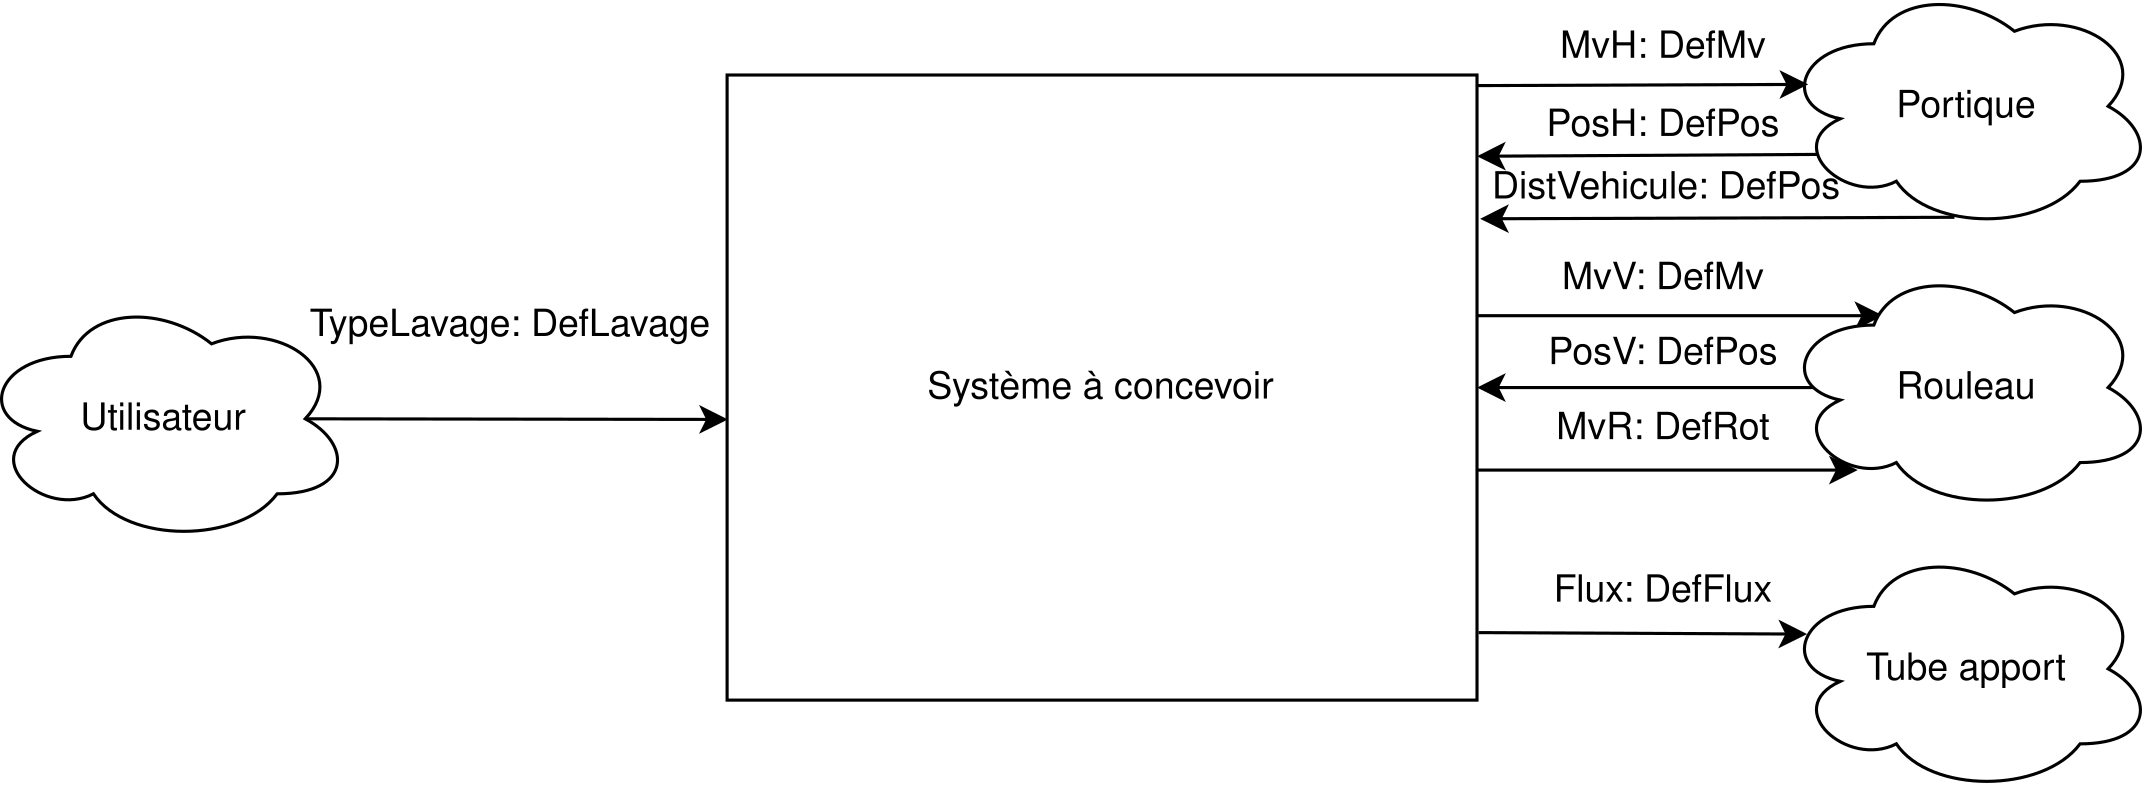
\includegraphics[width=1\linewidth]{entities.drawio.png}
	\caption{Entrées et sorties du circuit à concevoir}
	\label{fig:entrees_sorties_composant}
\end{figure}

Les entités Portique, Rouleau et Tube apport sont en réalité des sous-entité d'une "top" entité Système de lavage.
Pour clarifier la méthode et mieux regrouper les entrées/sorties selon leur cohérence, le choix a été fait de déconstruire cette entité peu spécifique.

\begin{figure}[H]
	\centering
	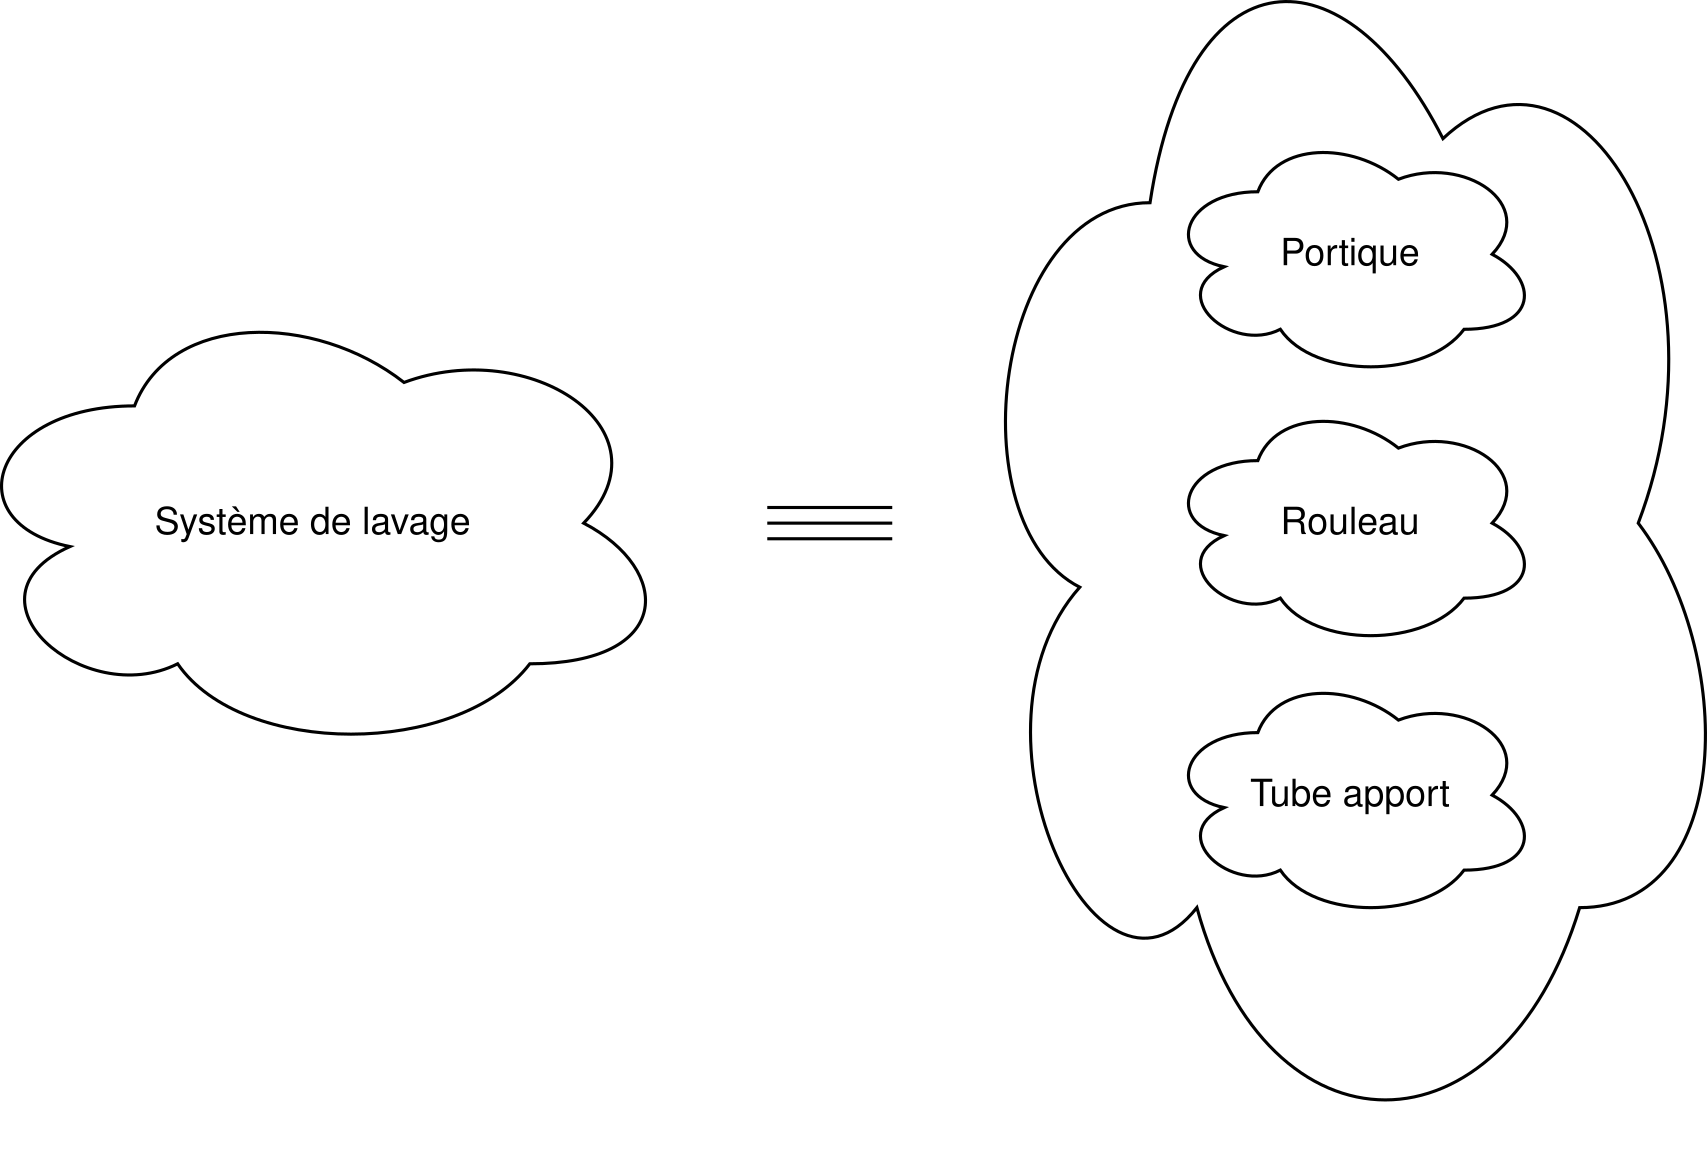
\includegraphics[width=0.7\linewidth]{topentity.drawio.png}
	\caption{Décomposition du Système de lavage}
	\label{fig:decomp_entities}
\end{figure}

\newpage

Le tableau ci-dessous récapitule les relations avec leur sens, leur catégorie et leur type.

\begin{table}[H]
	\centering
	\begin{tabular}{|c|c|c|c|c|}
		\hline
		Entités                       & Relation  & Catégorie    & Sens   & Type           \\
		\hline
		Utilisateur                   & TypeLavage  & Permanent    & Entrée   & DefLavage  \\
		\hline
		Portique                      & MvH  & Permanent    & Sortie   & DefMv             \\
									  & PosH  & Permanent    & Entrée   & DefPos           \\
									  & DistVehicule  & Permanent    & Entrée   & DefPos   \\
		\hline
		Rouleau                       & MvV  & Permanent    & Sortie   & DefMv             \\
									  & PosV  & Permanent    & Entrée   & DefPos           \\
									  & MvR  & Permanent    & Sortie   & DefRot            \\
    	\hline
		Tube apport                   & Flux  & Permanent    & Sortie   & DefFlux          \\
		\hline
	\end{tabular}
	\caption{Sens et rôle des signaux}
	\label{tab:entrees_sorties_composant}
\end{table}

Les différents types définis dans le tableau \ref{tab:entrees_sorties_composant} sont spécifiques à l'application.
Ils permettent de regrouper les informations essentielles qui doivent être échangées entre les entités et notre système.

\textbf{DefLavage} permet de définir le type de lavage lancé par l'utilisateur.
Il y a deux choix possibles: "Eau" ou "Produit". 
"Produit" est défini par défaut.

\textbf{DefMv} indique le mouvement horizontal de portique.
Le mouvement est défini par une vitesse.
DefMv est défini en m/s et peut prendre des valeurs positives ou négatives pour indiquer le sens de déplacement. 

\textbf{DefPos} définit la position d'une entité selon sa position d'origine.
C'est une valeur décimale définit en mètres.

\textbf{DefRot} définit la rotation du rouleau.
C'est un choix binaire entre: "Arrêté" et "Rotation".

\textbf{DefFlux} définit l'apport d'un élément par le tube d'apport.
C'est un choix entre: "Eau", "Produit" et "Air".

\newpage

\subsection{Spécifications fonctionnelles}
Les spécifications fonctionnelles comprennent la liste des fonctions du système
pour l'application (fonctions externes) et la description du comportement du système et
de l'environnement pour ces fonctions \cite{Calvez_2}.

\gap


\subsection{Spécifications opératoires}
\subsection{Spécifications technologiques}